\documentclass[12pt,letterpaper, onecolumn]{exam}
\usepackage{amsmath}
\usepackage{amssymb}
\usepackage{graphicx}
\usepackage[lmargin=71pt, tmargin=1.2in]{geometry}  %For centering solution box
\lhead{Leaft Header\\}
\rhead{Right Header\\}
% \chead{\hline} % Un-comment to draw line below header
\thispagestyle{empty}   %For removing header/footer from page 1

\begin{document}

\begingroup  
    \centering
    \LARGE STATS 212\\
    \LARGE Homework 2\\[0.5em]
    \large \today\\[0.5em]
    \large Samuel Molero\par
    \large samueljosemolero@tamu.edu\par
    \large Section: 501\par
\endgroup
\rule{\textwidth}{0.4pt}
\pointsdroppedatright   %Self-explanatory
\printanswers
\renewcommand{\solutiontitle}{\noindent\textbf{Ans:}\enspace}   %Replace "Ans:" with starting keyword in solution box

\begin{questions}
    \question Q1
    \begin{solution}
        \center 
        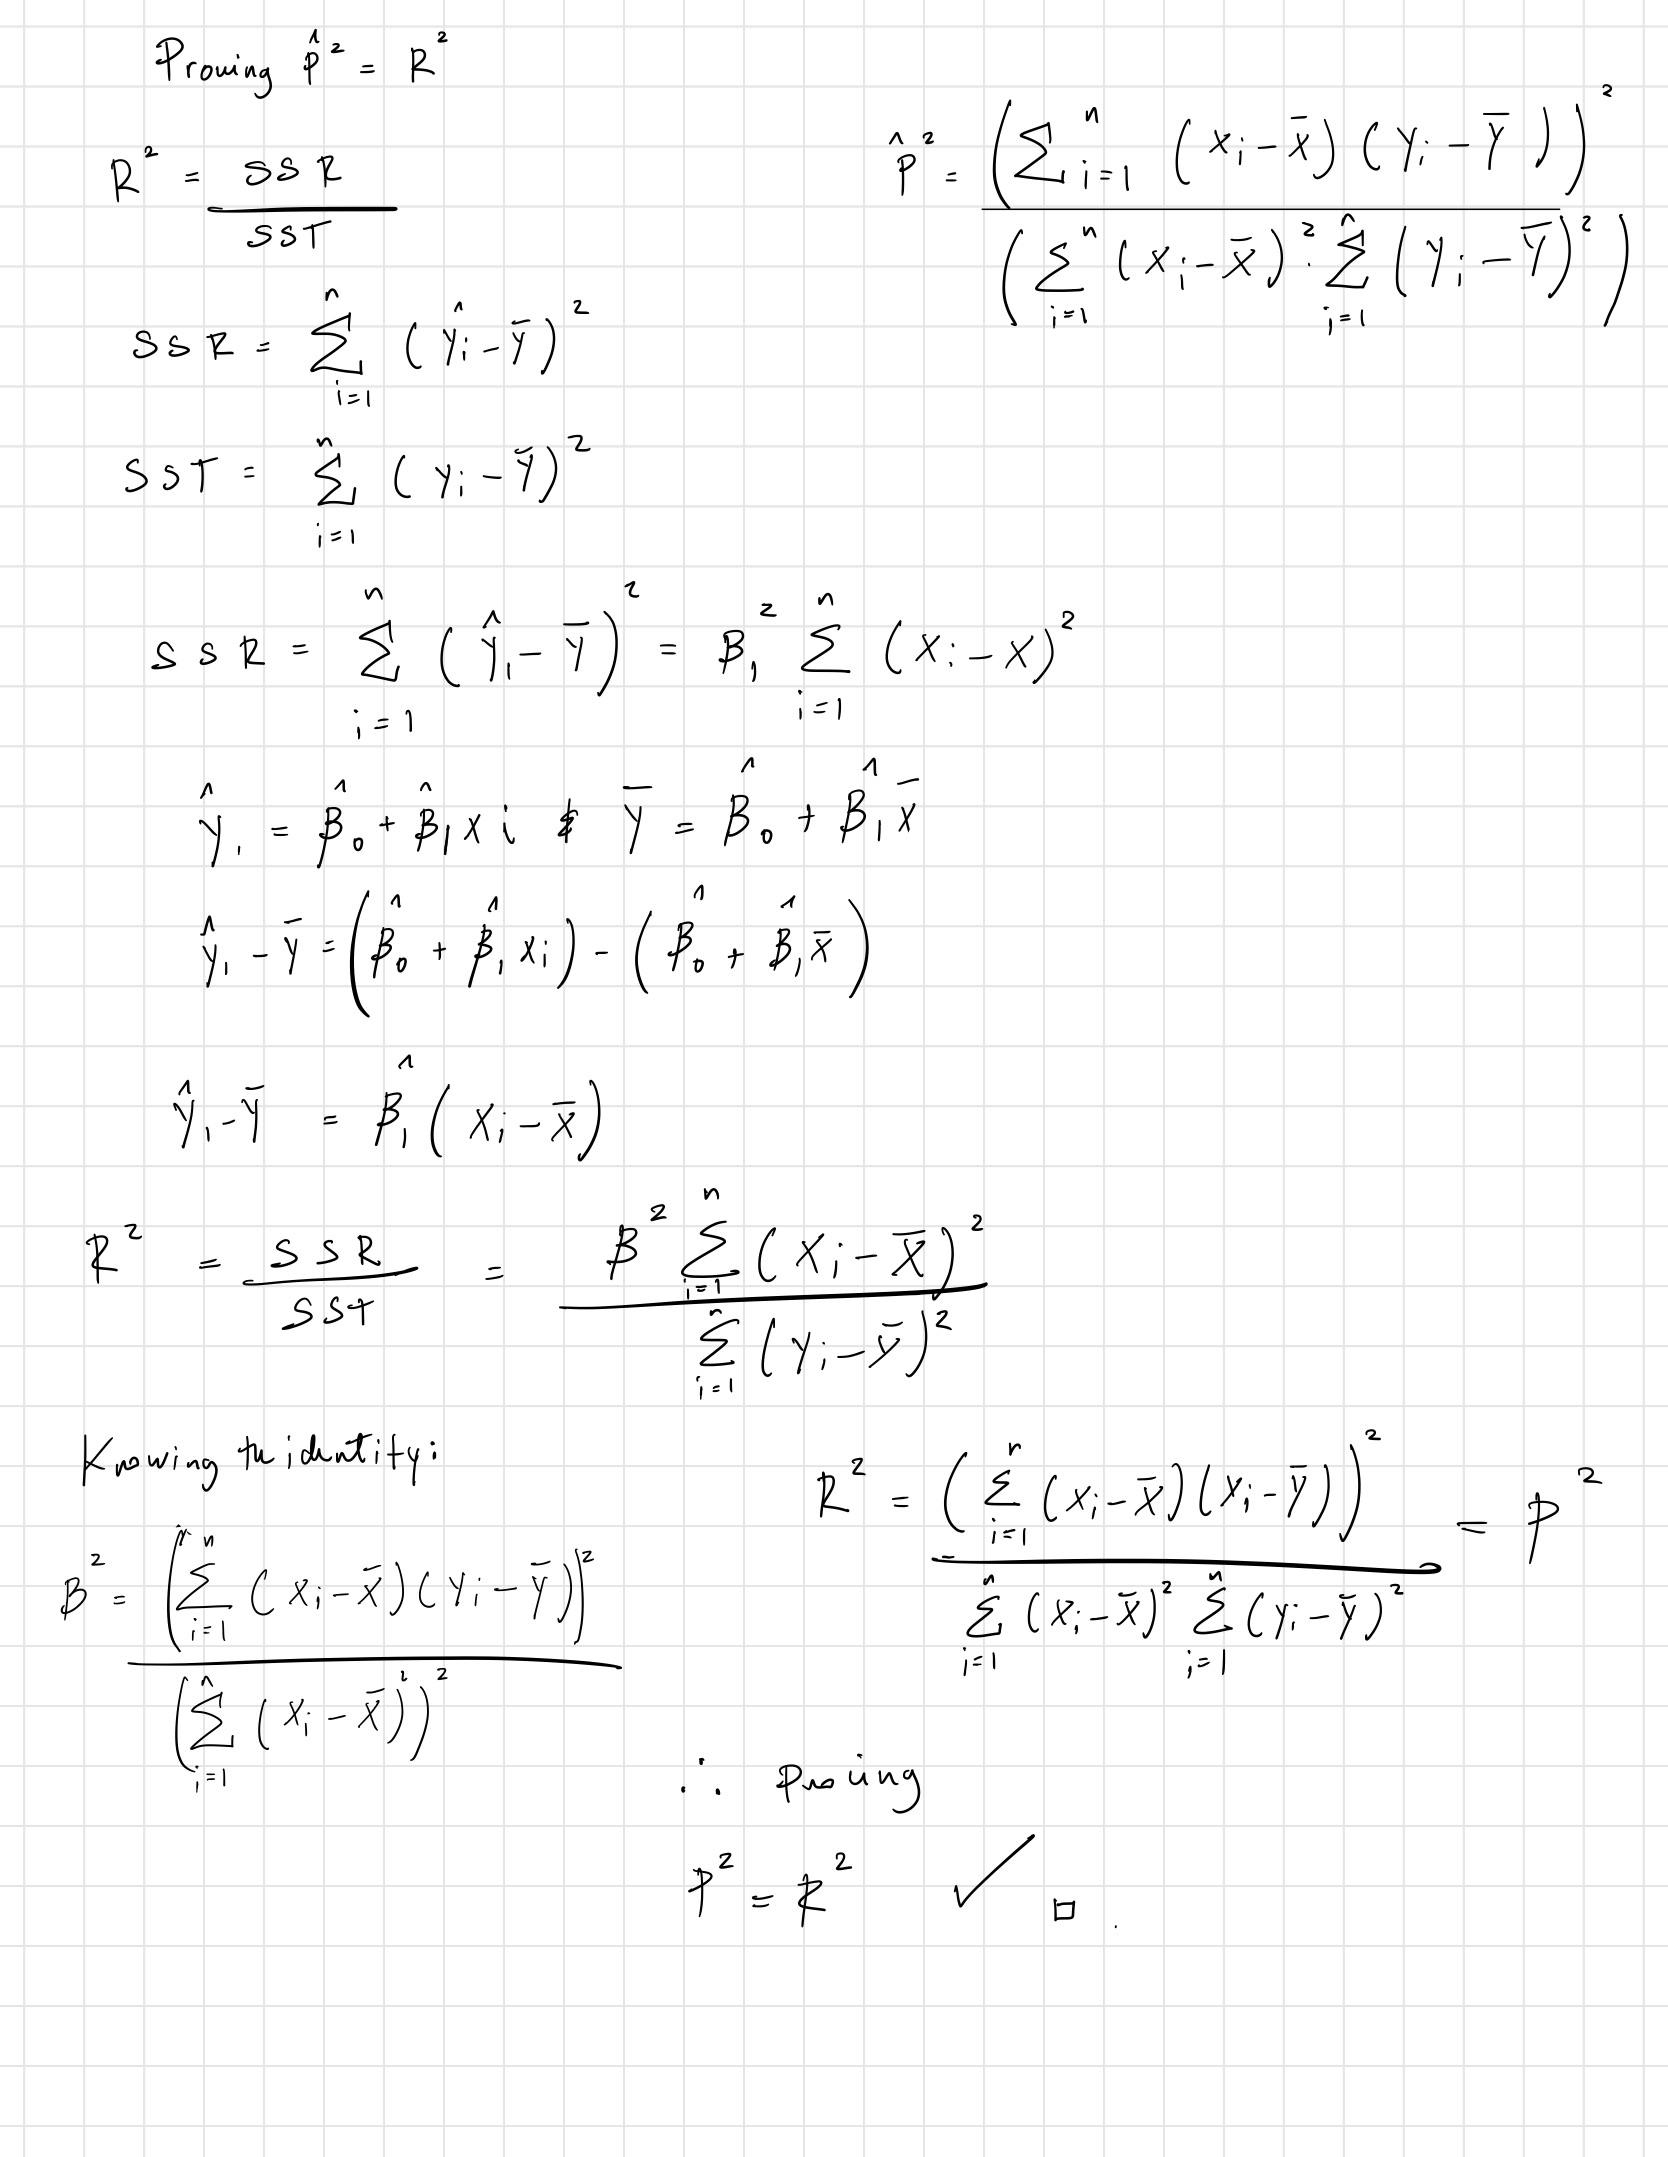
\includegraphics[width=0.7\textwidth]{Homeworks/ProvePR.jpg}
    \end{solution}

    \pagebreak
    \question Q2
    \begin{solution}
        \begin{parts}
            \part 
            \begin{verbatim}
             # AIC [239.5899 230.0744 231.8443 233.4604 
              235.2434 237.2078 234.6909 234.6980]
             # BIC [243.4774 235.2577 238.3235 241.2355 
             244.3142 247.5745 246.3534 247.6563]
            \end{verbatim}
            From the data collected after having created a good polynomial regression model from degrees 1 to 8, 
            the best degree for both AIC and BIC is 2.
            \part 
            \begin{verbatim}
            # tree_fit <- lm(y~poly(x, degree = 2, raw = TRUE))
            # summary(tree_fit)
            \end{verbatim}
            Running the following code will result in a P-value of $0.00154$, and since the P-value is less than $0.05$ the null is rejected and hence the coefficient of $x^{2}$ is significantly different from zero.
            \part 
                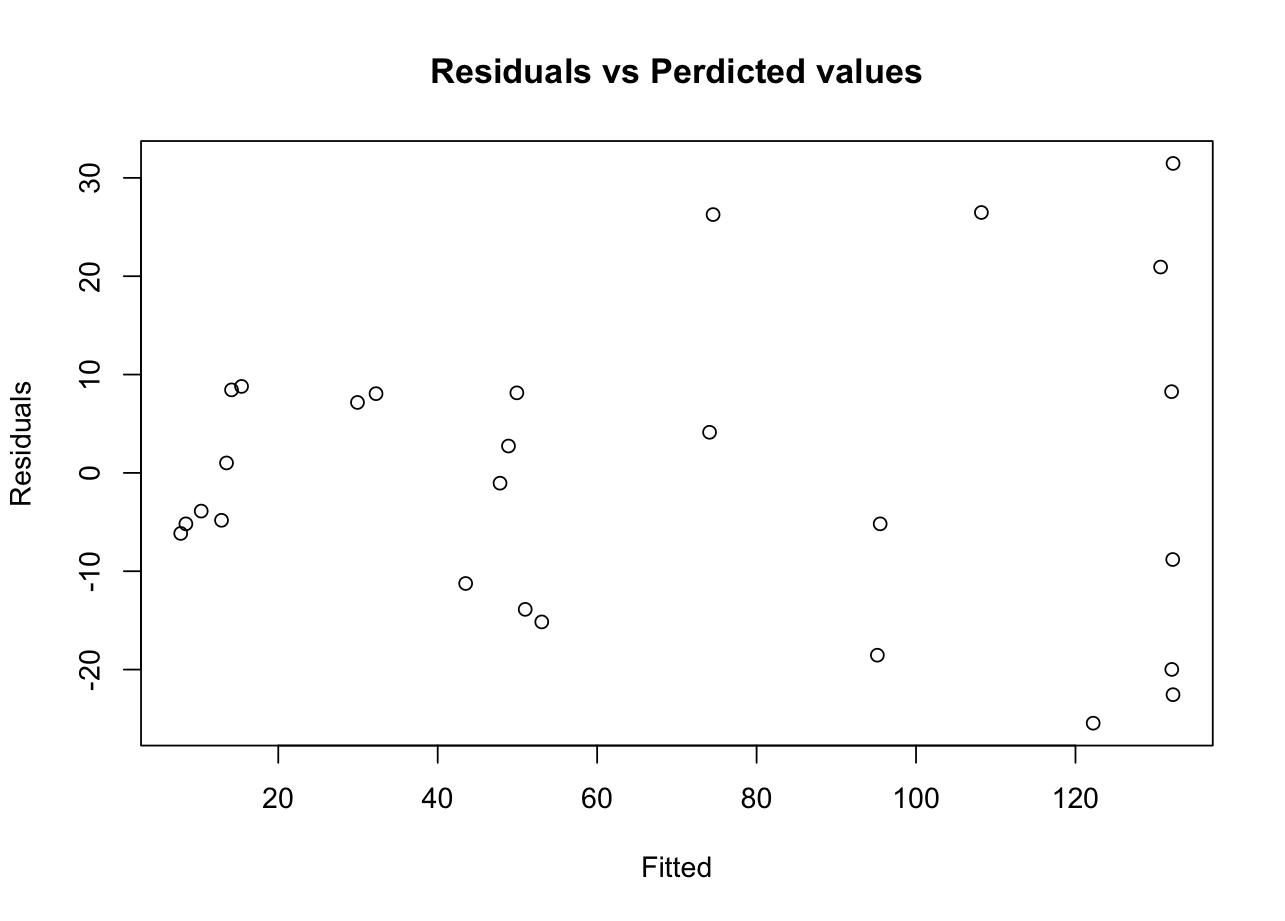
\includegraphics[width=0.8\textwidth]{Homeworks/RedVPred.png}\\
            What's remarkable about this graph, is that as the fitted values increase, the residuals tend to show greater variability, demonstrating that the spread of error is not constant and supporting the assumption that the coefficient of  $x^{2}$ is significantly different from zero.
               
            \part There is a 95\%\ confidence that the age of a tree with a 110 diameter is within the range $[18.17506, 84.82335]$.
        \end{parts}
    \end{solution}

    \pagebreak %Not necessary
    
   
  
\end{questions}
\end{document}